\documentclass[11pt,reqno,final]{amsart}

\pdfcompresslevel=0
\pdfobjcompresslevel=0

\usepackage[dvipsnames]{xcolor}% adds colors
\usepackage{amsmath, amsthm}% {amsfonts, amssymb}

% New Characters
\usepackage[latin1]{inputenc}%
\usepackage[T1]{fontenc}

\usepackage{MnSymbol}
\usepackage[normalem]{ulem}% underlining

\usepackage[theoremfont, largesc]{newpxtext} % different text,math font
\usepackage{newpxmath}

\makeatletter
\DeclareMathRadical{\sqrtsign}{symbols}{112}{largesymbols}{112}
% \let\sqrt=\undefined
% \DeclareRobustCommand\sqrt{\@ifnextchar[\@sqrt{\mathpalette\@x@sqrt}]}
% \def\@x@sqrt#1#2{%
%  \setbox\z@\hbox{$\m@th#1\sqrtsign{\mkern1mu #2}$}
%  \mkern3mu\box\z@}
\makeatother




% Page Typesetting
\usepackage[final]{microtype}
\usepackage{relsize}
\usepackage[margin=1in]{geometry}
\usepackage{framed}
\usepackage{tikz}
\usepackage{setspace}

\usepackage{hyperref}
\hypersetup{
  final,
  pdftitle={Math 135 - Continuity, Infinity},
  pdfauthor={Bonventre}, 
  linktoc=page,
  pagebackref,
  colorlinks=true,
  citecolor=PineGreen,
  linkcolor=PineGreen,
  linkbordercolor=PineGreen,
}


% Internal References

\usepackage[inline,shortlabels]{enumitem}

\numberwithin{equation}{section} 
\numberwithin{figure}{section}

\usepackage[nameinlink,capitalise,noabbrev]{cleveref}

\crefname{equation}{}{} % get \cref to behave as \eqref

% \theoremstyle{plain} % bold name, italic text
\newtheorem{theorem}[equation]{Theorem}%
\newtheorem*{theorem*}{Theorem}%
\newtheorem{lemma}[equation]{Lemma}%
\newtheorem{proposition}[equation]{Proposition}%
\newtheorem{corollary}[equation]{Corollary}%
\newtheorem{conjecture}[equation]{Conjecture}%
\newtheorem*{conjecture*}{Conjecture}%
\newtheorem{claim}[equation]{Claim}%
\newtheorem{question}{Question}

\theoremstyle{definition} % bold name, plain text
\newtheorem{definition}[equation]{Definition}%
\newtheorem*{definition*}{Definition}%
\newtheorem{example}[equation]{Example}%
\newtheorem*{example*}{Example}%
\newtheorem{remark}[equation]{Remark}%
\newtheorem{notation}[equation]{Notation}%
\newtheorem{convention}[equation]{Convention}%
\newtheorem{assumption}[equation]{Assumption}%
\newtheorem{exercise}[question]{Exercise}

% ---------- macros
\newcommand{\set}[1]{\left\{#1\right\}}%
\newcommand{\sets}[2]{\left\{ #1 \;|\; #2\right\}}%
\newcommand{\longto}{\longrightarrow}%
\newcommand{\into}{\hookrightarrow}%
\newcommand{\onto}{\twoheadrightarrow}%

\usepackage{harpoon}
\newcommand{\vect}[1]{\text{\overrightharp{\ensuremath{#1}}}}

\newcommand{\del}{\partial}%

\newcommand{\ki}{\chi}
\newcommand{\ksi}{\xi}
\newcommand{\Ksi}{\Xi}

\newcommand{\dlim}{\displaystyle\lim}

% %%%%%%%%%%%%%%%%%%%%%%%%%%%%%%%%%%%%%%%%%%%%%%%%%%%%%%%%%%%%%%%%%%%%%%%%%%%%%%%%%%%%%%%%%%%%%%%%%%%%

\begin{document}
\onehalfspacing

\begin{center}
        \textbf{\Large Math 135, Calculus 1, Fall 2020}\\[10pt]
        {\large 09-25: Continuity and Limits at Infinity}
\end{center}

\thispagestyle{empty}

\renewcommand{\thesection}{\Alph{section}}
\section{Continuity}

In many of the limit computations from 09-21 and 09-23, the function value and the limit values were different.
This is because, in general, \textit{the function value at $x=a$ has \textbf{no effect} on the limit of the function as $x \to a$.}
However, some functions are better behaved:
\begin{framed}
        A function $f(x)$ is \textit{continuous at $x=a$} if
        \[
                \dlim_{x \to a} f(x) = f(a).
        \]
\end{framed}

Intuitively:
\begin{itemize}
\item a function is continuous if it can be drawn without having to lift up your pencil.
\item A function is \textit{not} continuous if it has holes, jumps, asymptotes (infinite limits), or places where limits don't exist (e.g. infinite oscillations).
\end{itemize}

There are in fact \textit{three} conditions to check to say that $f(x)$ is continuous at $x=a$:
\begin{enumerate}[(1)]
\item $f(a)$ must exist
\item The limit as $x \to a$ of $f(x)$ must exist (in particular, it cannot be $\infty$ or $-\infty$).
\item The limit must equal the function value.
\end{enumerate}


\begin{example}
        Consider the function $f(x)$ with the following graph:
        \begin{center}
                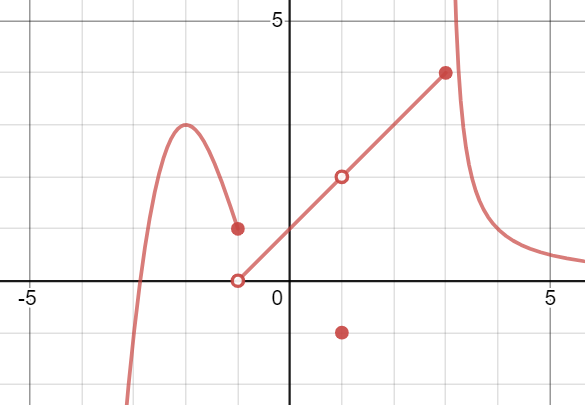
\includegraphics[width=2.4in]{09-25P_graph}
        \end{center}
        It is not continuous at $x=-1$, $x=1$, and $x=3$:
        \begin{itemize}
        \item it has a \textbf{jump discontinuity} at $x=-1$: both the left-handed and right-handed limits exist (and are finite), but they are note equal to each other.
        \item it has a \textbf{removable discontinuity} at $x=1$: $\lim_{x \to 1} f(x)$ exists (and equals 2), but this is \textit{different} from the function value $f(1) = 1$.
        \item it has an \textbf{infinite discontinuity} at $x=3$: (at least) one of the one-hand limits equals $\pm \infty$ (in this case $\lim_{x \to 3^+}f(x) = +\infty$).
        \end{itemize}
        Moreover, $f(x)$ is \textbf{left-continuous} at $x=-1$: the left-hand limit exists and equals the function value.
\end{example}

\begin{exercise}
        \begin{enumerate}[(a)]
        \item Is $f(x)$ \textbf{right-continuous} at $x=1$? Why or why not?
        \item Besides $x=-1$, where else is $f(x)$ left-continuous but not right-continuous?
        \end{enumerate}
\end{exercise}

\newpage

\begin{exercise}
        Consider the function $h(x)$ with the following graph, and fill in the following table
        (possible types: jump, removable, infinite, other).

        $ $
        \begin{minipage}{.5\textwidth}
                \begin{center}
                        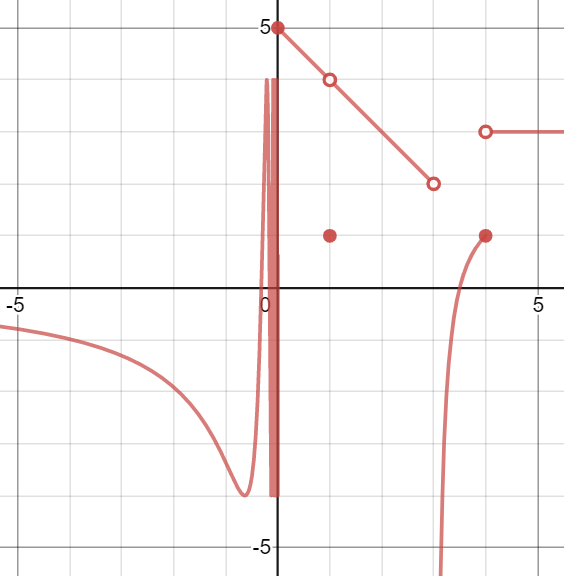
\includegraphics[width=2.5in]{09-25P_graph2.png}
                \end{center}
        \end{minipage}
        \begin{minipage}{.5\textwidth}
                {\renewcommand{\arraystretch}{2}%                
                  \begin{center}
                          \begin{tabular}{l|c|c}
                            discontinuity & \quad type \quad $ $& \quad left/right continuous? \\ \hline
                            $x=$ \qquad && \\
                            $x=$ && \\
                            $x=$ && \\
                            $x=$ &&\\
                          \end{tabular}
                  \end{center}
                }
        \end{minipage}
\end{exercise}

\begin{framed}
        \begin{itemize}
        \item Polynomials, rational functions, exponentials, logs, trig functions, and algebraic functions are \textit{all continuous on their domains} [See: Limit Law Overview, ``Direct Substitution Property''].
        \item Compositions of continuous functions are continuous.
        \end{itemize}
\end{framed}

\noindent To find limits of continuous functions, simply evaluate at the point in question (i.e. just plug in!).

\begin{exercise}
        Use continuity to find the value of $\dlim_{x \to 3} \log_5(\cos(t-3)+4)$.
        \vfill
\end{exercise}

\section{Limits at Infinity}

The expression $\dlim_{x \to \infty} f(x)$ means to calculate the function values of $f$ as $x$ gets larger and larger, and see if they approach a particular value. \\
As with other limits, possible answers include: a real number $L$, $\infty$, $-\infty$, or DNE.
\begin{example}
        $ $
        \begin{itemize}
        \item The infinite limit $\dlim_{x \to \infty}x^2 = \infty$, because as $x$ gets larger, $x^2$ grows ``without bound''.\\
        \item The infinite limit $\dlim_{x \to \infty} \dfrac{1}{x} = 0$, becuase as $x$ gets larger, $1/x$ gets smaller and smaller.
        \end{itemize}
\end{example}

We say that the function $f(x) = 1/x$ has a \textbf{horizontal asymptote} at $y = 0$, because the graph of $f$ approaches the horizontal line $y = 0$ as $x$ tends to $\infty$.

We can also take the limit to $-\infty$, and have horizontal asymptotes there:
\begin{example}
        We have
        \[
                \dlim_{x \to -\infty} x^2 = \infty,
                \qquad
                \dlim_{x \to -\infty} x^3 = -\infty,
                \qquad
                \dlim_{x \to -\infty} e^x = 0.
        \]
        So $f(x) = e^x$ has a horizontal asymptote at $y = 0$.
\end{example}

\newpage

\begin{exercise}
        Evaluate each of the following limits, if they exist.
        \begin{enumerate}[(a)]\itemsep+15pt
        \item $\dlim_{x \to \infty} e^{2x}$
        \item $\dlim_{x \to \infty} e^{-2x}$
        \item $\dlim_{x \to -\infty} e^{2x}$
        \item $\dlim_{x \to \infty} -x^4 + 3x^2 + 7$
        \item $\dlim_{x \to \infty} \sin x$
        \item $\dlim_{x \to -\infty} 2x^2- 3x^3$
        \item $\dlim_{x \to \infty} \tan^{-1}x$
        \item $\dlim_{x \to -\infty} \tan^{-1}x$
        \end{enumerate}
\end{exercise}

\subsection*{Infinite limits of rational functions}

\begin{example}
        Consider the limit limit $\dlim_{x \to \infty} \dfrac{3x^3+5x-2}{4x^2+7}$.
        If we simply ``plug in'', we get $\infty/\infty$, which is an \textbf{indeterminant form} (more on Monday).
        Instead, let's divide the top and bottom of the fraction by the \textbf{highest power in the demoninator}, which in this case is $x^2$. This gives:
        \[
                \dlim_{x \to \infty} \dfrac{3x^3+5x-2}{4x^2+7} =
                \dlim_{x \to \infty} \dfrac{\frac{3x^3}{x^2}+\frac{5x}{x^2}-\frac{2}{x^2}}{\frac{4x^2}{x^2}+\frac{7}{x^2}} =
                \dlim_{x \to \infty} \dfrac{3+ \frac{5}{x} - \frac{2}{x^2}}{4 + \frac{7}{x^2}} =
                \dfrac{3}{4}.
        \]        
\end{example}

\begin{exercise}
        Evaluate $\dlim_{x \to \infty} \dfrac{6x^4-5x^3+2x}{4x^2-7x^4+1}$.
        \vfill
\end{exercise}

\begin{exercise}
        Evaluate $\dlim_{x \to \infty} \dfrac{6x^4-5x^3+2x}{4x^5-7x^4+1}$.
        \vfill
\end{exercise}

\begin{exercise}
        Evaluate $\dlim_{x \to \infty} \dfrac{\sqrt{25x^4+10}}{3x^2+1}$.
        \textit{Hint: ignore the 10 in the numerator.}
        \vfill
\end{exercise}

\end{document}
